\documentclass[11pt,a4paper]{article}

\usepackage[utf8]{inputenc}
\usepackage[T1]{fontenc}
\usepackage[margin=1in]{geometry}
\usepackage{array}
\usepackage{booktabs}
\usepackage{caption}
\usepackage{enumitem}
\usepackage{float}
\usepackage{graphicx}
\usepackage{hyperref}
\usepackage{listings}
\usepackage{microtype}
\usepackage{pdfpages}
\usepackage{tabularx}
\usepackage[table]{xcolor}
\usepackage{xurl}
\usepackage{tikz}
\usetikzlibrary{arrows.meta,calc,fit,positioning,shapes.geometric}

\hypersetup{
  colorlinks=true,
  linkcolor=black,
  urlcolor=blue!50!black,
  citecolor=black
}

\definecolor{ituBlue}{RGB}{0,64,128}
\definecolor{softBlue}{RGB}{226,239,255}
\definecolor{softGreen}{RGB}{226,246,232}
\definecolor{softOrange}{RGB}{255,239,214}
\definecolor{softGray}{RGB}{243,245,247}
\definecolor{codeBackground}{RGB}{247,247,244}
\definecolor{codeKeyword}{RGB}{0,55,140}
\definecolor{codeComment}{RGB}{65,115,80}

\lstset{
  backgroundcolor=\color{codeBackground},
  basicstyle=\ttfamily\footnotesize,
  breaklines=true,
  captionpos=b,
  columns=fullflexible,
  commentstyle=\color{codeComment}\itshape,
  frame=single,
  keepspaces=true,
  keywordstyle=\color{codeKeyword}\bfseries,
  numbers=left,
  numbersep=8pt,
  numberstyle=\scriptsize\color{gray},
  showspaces=false,
  showstringspaces=false,
  tabsize=2
}

\newcommand{\projecttitle}{STM32N6570-DK Based Licence Plate Detection and Secure Snapshot Transfer System}
\newcommand{\coursename}{ELE529E Final Project}
\newcommand{\snapshotgraphic}{%
  \IfFileExists{snapshot.png}{%
    
\includegraphics[width=0.76\textwidth]{snapshot.png}%
  }{%
    \IfFileExists{../snapshot.png}{%
      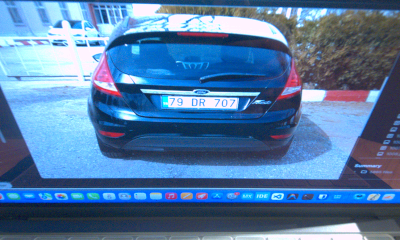
\includegraphics[width=0.76\textwidth]{../snapshot.png}%
    }{%
      \fbox{\parbox[c][4cm][c]{0.76\textwidth}{\centering Snapshot image not found.}}%
    }%
  }%
}
\newcommand{\memoryutilizationgraphic}{%
  \IfFileExists{memory_utilization.png}{%
    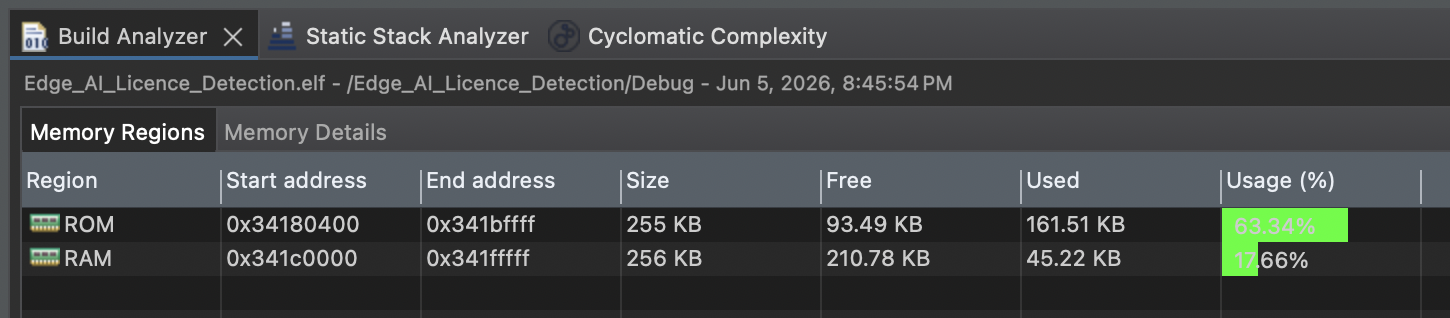
\includegraphics[width=0.95\textwidth]{memory_utilization.png}%
  }{%
    \IfFileExists{Docs/memory_utilization.png}{%
      
\includegraphics[width=0.95\textwidth]{Docs/memory_utilization.png}%
    }{%
      \fbox{\parbox[c][3cm][c]{0.95\textwidth}{\centering Memory utilization image not found.}}%
    }%
  }%
}
\newcommand{\driverunittestreportpdf}{%
  \IfFileExists{c_driver_unit_test_report.pdf}{%
    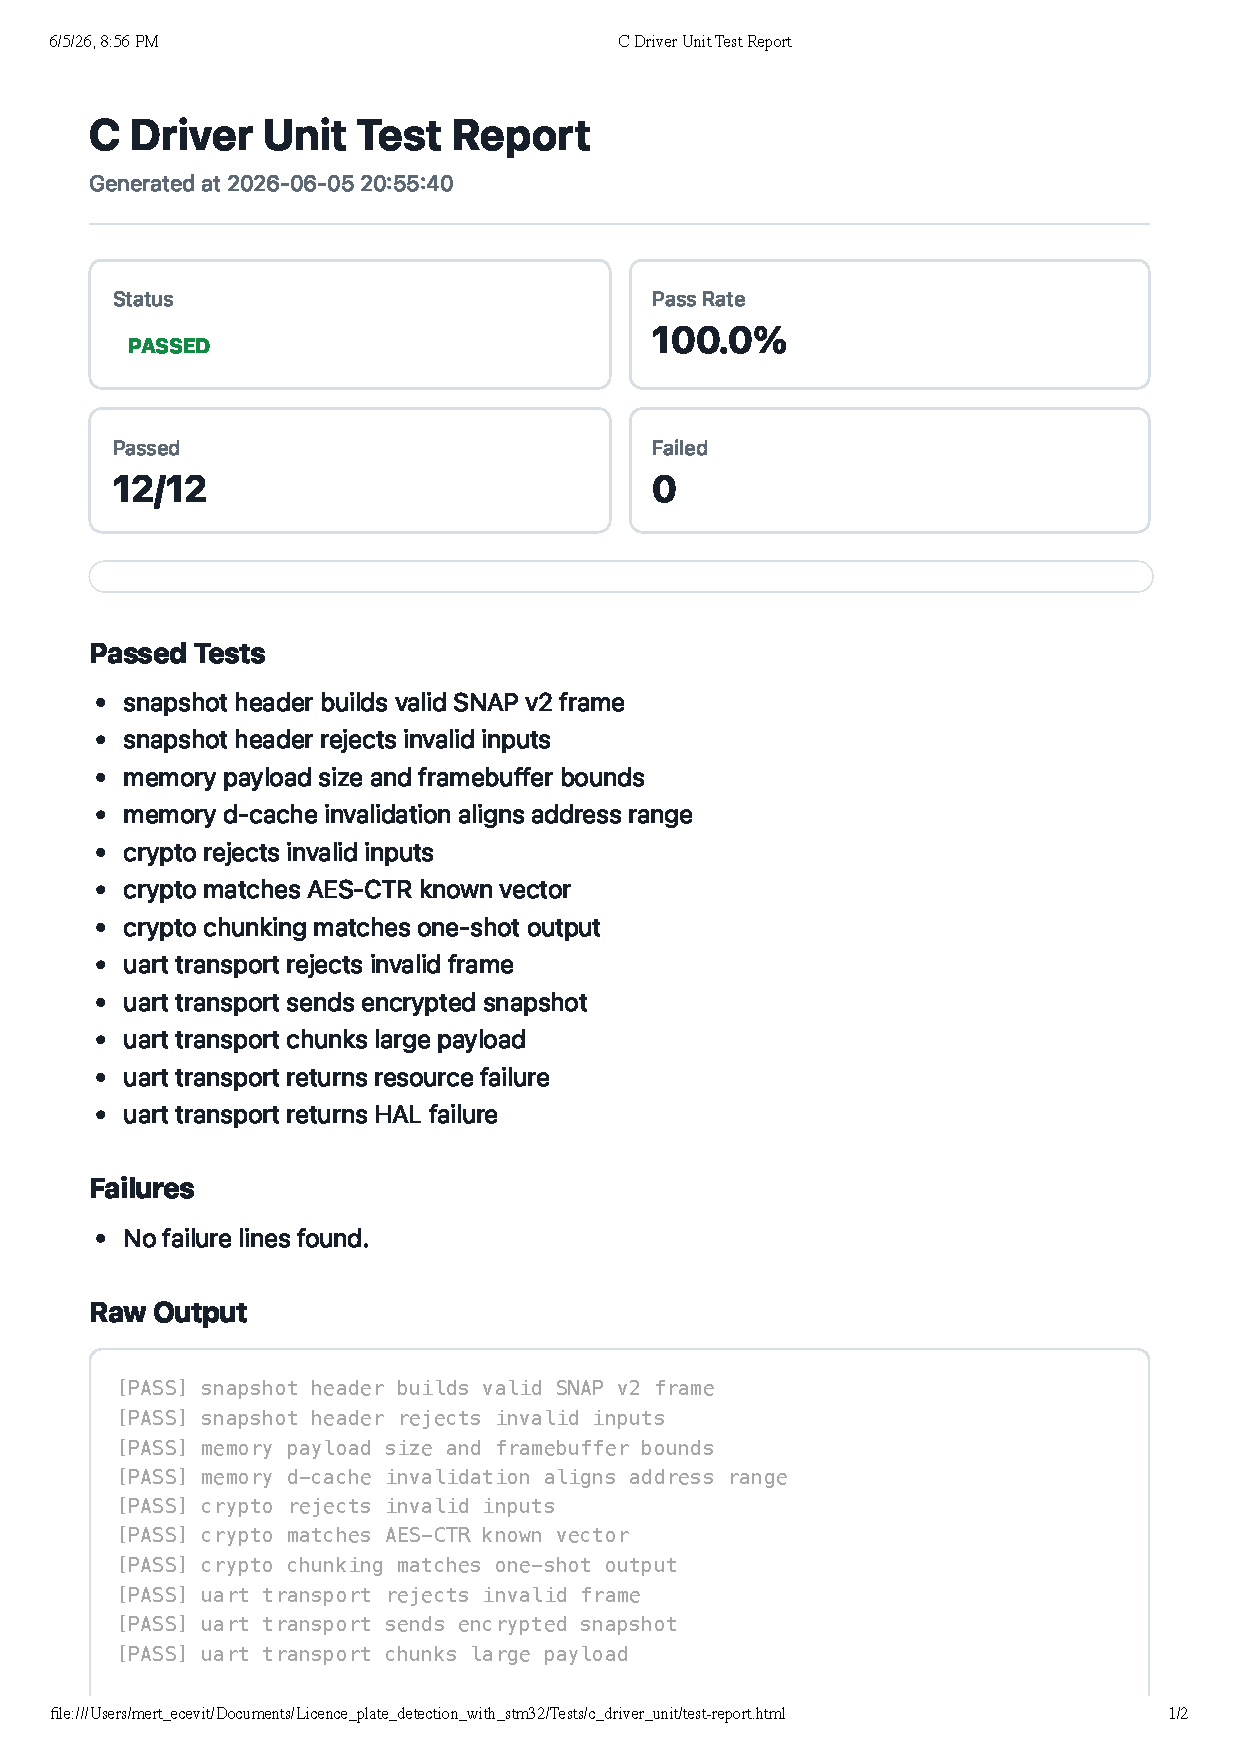
\includepdf[pages=-,pagecommand={},scale=0.92]{c_driver_unit_test_report.pdf}%
  }{%
    \IfFileExists{Docs/c_driver_unit_test_report.pdf}{%
      
\includepdf[pages=-,pagecommand={},scale=0.92]{Docs/c_driver_unit_test_report.pdf}%
    }{%
      \noindent\fbox{\parbox[c][4cm][c]{0.95\textwidth}{\centering C driver unit test report PDF not found.}}%
    }%
  }%
}

\begin{document}

\begin{titlepage}
  \centering
  \vspace*{1.0cm}
  {\Large\bfseries Istanbul Technical University\par}
  \vspace{0.25cm}
  {\large MSc. Program in Electronics Engineering\par}
  \vspace{1.6cm}
  {\color{ituBlue}\rule{\textwidth}{1.2pt}\par}
  \vspace{0.55cm}
  {\LARGE\bfseries \projecttitle\par}
  \vspace{0.35cm}
  {\Large\bfseries Final Project Report\par}
  \vspace{0.55cm}
  {\color{ituBlue}\rule{\textwidth}{1.2pt}\par}
  \vspace{1.2cm}
  \begin{tabularx}{\textwidth}{>{\raggedleft\arraybackslash}p{3.2cm}>{\raggedright\arraybackslash}X}
    \textbf{Course:} & \coursename \\
    \textbf{Platform:} & STM32N6570-DK, Cortex-M55, IMX335 camera, RK050HR18 LCD \\
    \textbf{Repository:} & \url{https://github.com/MertEcevit-ops/Licence_plate_detection_with_stm32} \\
    \textbf{Date:} & June 2026
  \end{tabularx}
  \vfill
  \begin{tabular}{ll}
    \toprule
    \textbf{Student} & \textbf{Student ID} \\
    \midrule
    Yusuf Tekin & 504251281 \\
    Mert Ecevit & 504251050 \\
    \bottomrule
  \end{tabular}
  \vspace*{1.0cm}
\end{titlepage}

\pagenumbering{roman}
\tableofcontents
\newpage
\pagenumbering{arabic}

\section{Abstract}
This report presents the final design and implementation of a licence plate
detection project built around the STM32N6570-DK board. The current embedded
software captures camera frames with the IMX335 image sensor and DCMIPP
pipeline, warms up the ISP, captures a decimated RGB565 snapshot, encrypts the
snapshot payload with AES-128-CTR, and streams the frame to a host computer over
UART using a deterministic binary protocol. The host-side tooling validates the
protocol, decrypts the payload, converts RGB565 pixels to RGB888, and stores a
standard image file. A separate Python ALPR pipeline using YOLO and EasyOCR is
included for licence plate detection and text recognition on host-side images.

\section{Project Scope and Objectives}
The project objective is to create an end-to-end embedded vision demonstrator
for licence plate detection on STM32 hardware. The final implementation focuses
on a reliable camera-to-host snapshot path, because this path is the foundation
needed before moving heavier ALPR inference fully onto the embedded target.

\begin{tabularx}{\textwidth}{@{}lX@{}}
\toprule
\textbf{Goal} & \textbf{Final implementation status} \\
\midrule
Camera acquisition & IMX335 sensor probing, DCMIPP configuration, ISP warmup, RGB565 framebuffer capture. \\
Display bring-up & LTDC layer configured on the RK050HR18 display using the shared framebuffer. \\
Host transfer & Button-triggered snapshot transfer over COM1 UART at 115200 baud. \\
Security & AES-128-CTR stream encryption for the image payload, keyed identically in firmware and host code. \\
Protocol robustness & Fixed-size v2 header, magic-byte resynchronization, strict dimension and payload-size validation. \\
ALPR software & Host Python pipeline with YOLO plate detection, EasyOCR recognition, and Turkish plate-format normalization. \\
\bottomrule
\end{tabularx}

\section{System Overview}
The system is split into two cooperating parts. The embedded firmware is
responsible for deterministic camera capture, resource ownership, display
configuration, encryption, and serial transmission. The host application is
responsible for receiving the frame, decrypting it, converting it into a
standard RGB image, and optionally feeding images into the ALPR inference
pipeline.

\begin{figure}[H]
\centering
\resizebox{\textwidth}{!}{%
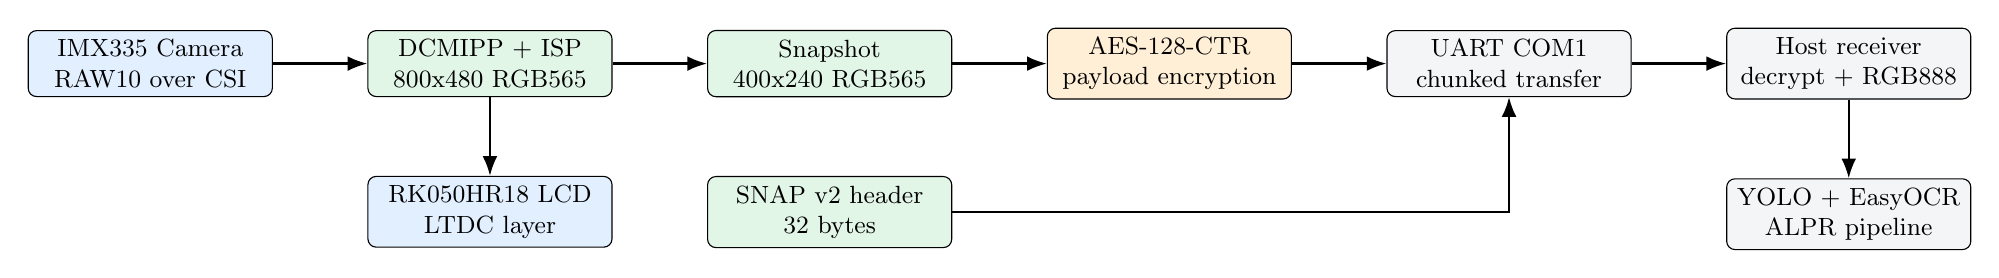
\begin{tikzpicture}[
  node distance=1.1cm and 1.2cm,
  block/.style={draw, rounded corners=3pt, minimum width=3.1cm, minimum height=0.8cm, align=center, font=\small},
  hw/.style={block, fill=softBlue},
  fw/.style={block, fill=softGreen},
  sec/.style={block, fill=softOrange},
  host/.style={block, fill=softGray},
  arrow/.style={-{Latex[length=2.5mm]}, thick}
]
  \node[hw] (sensor) {IMX335 Camera\\RAW10 over CSI};
  \node[fw, right=of sensor] (dcmipp) {DCMIPP + ISP\\800x480 RGB565};
  \node[fw, right=of dcmipp] (snapshot) {Snapshot\\400x240 RGB565};
  \node[sec, right=of snapshot] (crypto) {AES-128-CTR\\payload encryption};
  \node[fw, below=1.0cm of snapshot] (protocol) {SNAP v2 header\\32 bytes};
  \node[host, right=of crypto] (uart) {UART COM1\\chunked transfer};
  \node[host, right=of uart] (receiver) {Host receiver\\decrypt + RGB888};
  \node[host, below=1.0cm of receiver] (alpr) {YOLO + EasyOCR\\ALPR pipeline};
  \node[hw, below=1.0cm of dcmipp] (lcd) {RK050HR18 LCD\\LTDC layer};

  \draw[arrow] (sensor) -- (dcmipp);
  \draw[arrow] (dcmipp) -- (snapshot);
  \draw[arrow] (snapshot) -- (crypto);
  \draw[arrow] (crypto) -- (uart);
  \draw[arrow] (uart) -- (receiver);
  \draw[arrow] (receiver) -- (alpr);
  \draw[arrow] (protocol) -| (uart);
  \draw[arrow] (dcmipp) -- (lcd);
\end{tikzpicture}%
}
\caption{End-to-end data path implemented in the project.}
\label{fig:system_overview}
\end{figure}

\section{Hardware and Software Platform}
\begin{itemize}[noitemsep]
  \item \textbf{Development board:} STM32N6570-DK.
  \item \textbf{MCU family:} STM32N657X0H3QU, Cortex-M55 class target.
  \item \textbf{Camera:} IMX335 image sensor configured as RAW10 over CSI.
  \item \textbf{Display:} RK050HR18 panel driven through LTDC.
  \item \textbf{RTOS:} FreeRTOS with a dedicated camera task.
  \item \textbf{Host environment:} Python 3 tooling under \texttt{Tools/}.
  \item \textbf{ALPR models:} YOLO \texttt{.pt} detector files and \texttt{emnist\_ocr.h5} model artifact are stored in the repository.
\end{itemize}

\section{Firmware Architecture}
The firmware is organized into small application modules rather than keeping all
logic in \texttt{main.c}. This separation makes the capture path easier to test
and keeps ownership of shared hardware explicit.

\begin{tabularx}{\textwidth}{@{}lX@{}}
\toprule
\textbf{Module} & \textbf{Responsibility} \\
\midrule
\texttt{app\_platform} & Initializes LEDs, USER1 button, and COM1 UART logging/transport settings. \\
\texttt{app\_camera} & Probes IMX335, initializes DCMIPP, runs ISP warmup, configures decimation, captures snapshots. \\
\texttt{app\_ltdc} & Initializes LTDC timing and maps the framebuffer to layer 1. \\
\texttt{app\_resources} & Provides FreeRTOS mutexes for camera, UART, and framebuffer ownership. \\
\texttt{app\_memory} & Computes RGB565 payload sizes, bounds-checks framebuffer access, invalidates D-cache safely. \\
\texttt{app\_crypto} & Implements AES-128 block encryption and CTR-mode payload streaming. \\
\texttt{snapshot\_protocol} & Builds the fixed 32-byte SNAP v2 frame header. \\
\texttt{app\_transport\_uart} & Sends the header and encrypted payload in 4096-byte UART chunks. \\
\bottomrule
\end{tabularx}

\subsection{Runtime Flow}
Only one application task is created by \texttt{AppTasks\_Create}. The task
warms up the camera pipeline, switches to decimated snapshot mode, then waits
for the USER1 button before each capture and transfer.

\begin{figure}[H]
\centering
\resizebox{0.9\textwidth}{!}{%
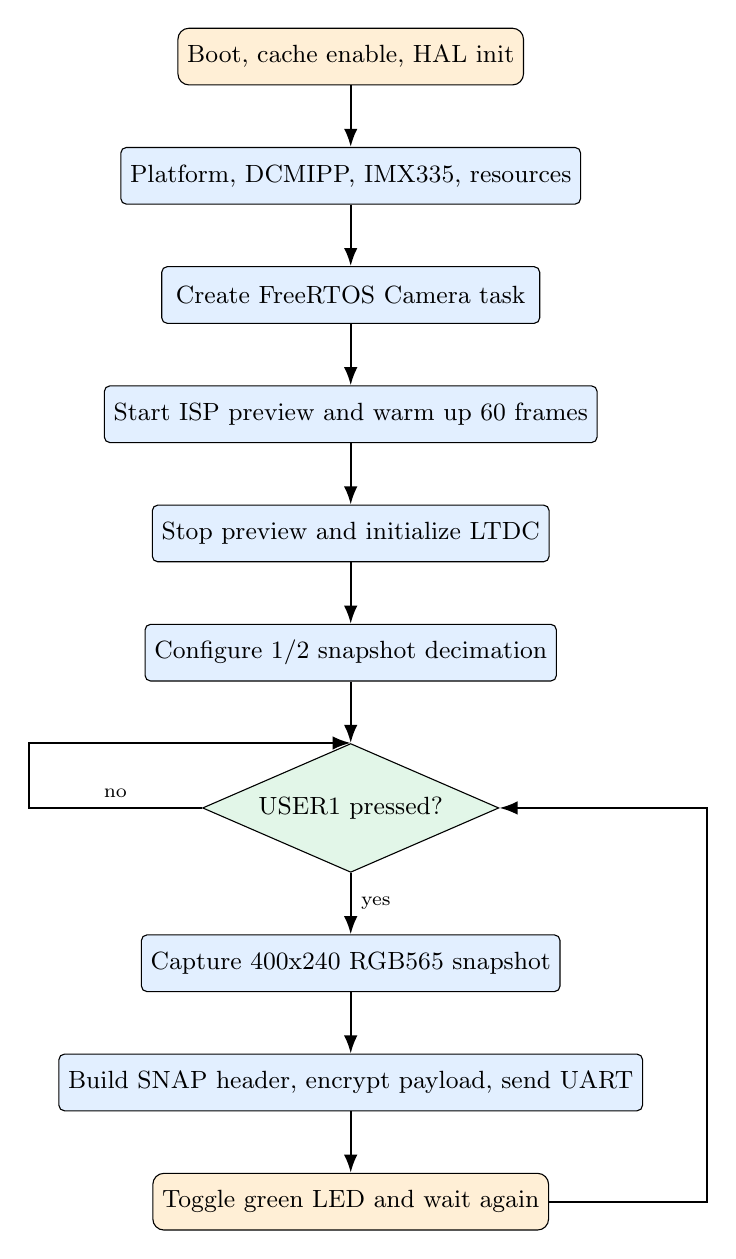
\begin{tikzpicture}[
  node distance=0.78cm,
  startstop/.style={draw, rounded corners=4pt, minimum width=3.6cm, minimum height=0.72cm, align=center, fill=softOrange, font=\small},
  process/.style={draw, rounded corners=2pt, minimum width=4.8cm, minimum height=0.72cm, align=center, fill=softBlue, font=\small},
  decision/.style={draw, diamond, aspect=2.3, minimum width=2.9cm, align=center, fill=softGreen, font=\small},
  arrow/.style={-{Latex[length=2.3mm]}, thick}
]
  \node[startstop] (boot) {Boot, cache enable, HAL init};
  \node[process, below=of boot] (init) {Platform, DCMIPP, IMX335, resources};
  \node[process, below=of init] (task) {Create FreeRTOS Camera task};
  \node[process, below=of task] (preview) {Start ISP preview and warm up 60 frames};
  \node[process, below=of preview] (stop) {Stop preview and initialize LTDC};
  \node[process, below=of stop] (dec) {Configure 1/2 snapshot decimation};
  \node[decision, below=of dec] (button) {USER1 pressed?};
  \node[process, below=of button] (capture) {Capture 400x240 RGB565 snapshot};
  \node[process, below=of capture] (send) {Build SNAP header, encrypt payload, send UART};
  \node[startstop, below=of send] (done) {Toggle green LED and wait again};

  \draw[arrow] (boot) -- (init);
  \draw[arrow] (init) -- (task);
  \draw[arrow] (task) -- (preview);
  \draw[arrow] (preview) -- (stop);
  \draw[arrow] (stop) -- (dec);
  \draw[arrow] (dec) -- (button);
  \draw[arrow] (button) -- node[right, font=\scriptsize]{yes} (capture);
  \draw[arrow] (capture) -- (send);
  \draw[arrow] (send) -- (done);
  \draw[arrow] (done.east) -- ++(2.0,0) |- (button.east);
  \draw[arrow] (button.west) -- node[above, font=\scriptsize]{no} ++(-2.2,0) |- (button.north);
\end{tikzpicture}%
}
\caption{Firmware activity diagram for one snapshot cycle.}
\label{fig:runtime_flow}
\end{figure}

\subsection{FreeRTOS Multitasking and Resource Ownership}
The firmware uses FreeRTOS to separate the time-sensitive camera workflow from
the initialization path in \texttt{main.c}. After cache, HAL, platform, DCMIPP,
camera sensor, and resource initialization complete, \texttt{AppTasks\_Create}
creates a dedicated \texttt{Camera} task. The scheduler is then started through
\texttt{AppTasks\_StartScheduler}, so the capture loop runs as an RTOS task
instead of a blocking bare-metal loop.

\begin{table}[H]
\centering
\begin{tabularx}{0.96\textwidth}{@{}l l X@{}}
\toprule
\textbf{Execution context} & \textbf{Priority / timing} & \textbf{Role} \\
\midrule
\texttt{Camera} task & \texttt{tskIDLE\_PRIORITY + 3}, stack size 2048 & Runs ISP warmup, waits for USER1, captures snapshots, encrypts payloads, and starts UART transmission. \\
FreeRTOS delay points & 1 ms, 10 ms, and 30 ms waits & Yield CPU time during ISP background processing, snapshot timeout polling, and button debounce. \\
DCMIPP callbacks & HAL event context & Increment the frame counter used by the task to detect preview/snapshot completion. \\
Resource mutexes & Camera, UART, framebuffer & Serialize shared hardware ownership and keep the design ready for additional tasks or transport paths. \\
\bottomrule
\end{tabularx}
\caption{Multitasking and synchronization structure used by the firmware.}
\label{tab:multitasking}
\end{table}

Although the current application creates one main camera task, the architecture
is intentionally RTOS-oriented. The camera, UART, and framebuffer are protected
by mutexes in \texttt{app\_resources}; this prevents overlapping access during
capture and transfer, and it keeps future expansion straightforward if a
separate logging, communication, or inference task is added. Button waiting and
snapshot polling use \texttt{vTaskDelay}, so the task does not busy-wait while
the scheduler is active.

\section{Snapshot Communication Protocol}
The board sends each image as a deterministic binary frame. All integer fields
are little-endian. The image payload is RGB565 before encryption and AES-128-CTR
ciphertext on the wire when the AES flag is set.

\begin{table}[H]
\centering
\begin{tabularx}{0.98\textwidth}{@{}r r l X@{}}
\toprule
\textbf{Offset} & \textbf{Size} & \textbf{Field} & \textbf{Meaning} \\
\midrule
0 & 4 & \texttt{magic} & ASCII \texttt{SNAP}. \\
4 & 1 & \texttt{version} & Protocol version, currently \texttt{2}. \\
5 & 1 & \texttt{header\_size} & Header size, currently 32 bytes. \\
6 & 1 & \texttt{pixel\_format} & \texttt{1} means RGB565. \\
7 & 1 & \texttt{flags} & Bit \texttt{0x02} means AES-128-CTR encrypted payload. \\
8 & 2 & \texttt{width} & Snapshot width after decimation, currently 400. \\
10 & 2 & \texttt{height} & Snapshot height after decimation, currently 240. \\
12 & 2 & \texttt{bytes\_per\_pixel} & RGB565 uses 2 bytes per pixel. \\
14 & 2 & \texttt{decimation} & Current factor is 2. \\
16 & 4 & \texttt{payload\_size} & \texttt{width * height * bytes\_per\_pixel}. \\
20 & 4 & \texttt{frame\_id} & Monotonic frame counter used in the CTR counter block. \\
24 & 4 & reserved & Reserved, currently zero. \\
28 & 4 & reserved & Reserved, currently zero. \\
32 & variable & payload & AES-128-CTR ciphertext for the RGB565 frame. \\
\bottomrule
\end{tabularx}
\caption{SNAP v2 UART frame layout implemented by firmware and host tooling.}
\label{tab:protocol}
\end{table}

\section{Security and Robustness}
The implemented security layer is lightweight and appropriate for a serial
snapshot demonstrator. The payload is encrypted using AES-128 in CTR mode. The
firmware derives the counter from a fixed nonce, the frame ID, and a block
counter; the Python host mirrors the same operation so encryption and decryption
use the same function.

Robustness is handled through deterministic sizes and explicit validation:
\begin{itemize}[noitemsep]
  \item The receiver scans byte-by-byte until the \texttt{SNAP} magic appears.
  \item The host rejects unsupported protocol versions, header sizes, pixel formats, invalid dimensions, and payload-size mismatches.
  \item The firmware validates framebuffer bounds before invalidating cache or transmitting data.
  \item UART and framebuffer access are serialized with FreeRTOS mutexes.
  \item The payload is streamed in fixed 4096-byte chunks, so no full-frame copy is allocated for transmission.
\end{itemize}

\section{Memory Utilization}
The STM32CubeIDE Build Analyzer output in Figure~\ref{fig:memory_utilization}
shows that the linked firmware image remains within the configured ROM and RAM
regions. ROM usage is 161.51 KB out of 255 KB, corresponding to 63.34 percent.
RAM usage is 45.22 KB out of 256 KB, corresponding to 17.66 percent, leaving
210.78 KB free in the reported RAM region.

\begin{figure}[H]
\centering
\memoryutilizationgraphic
\caption{Build Analyzer memory utilization for the firmware image.}
\label{fig:memory_utilization}
\end{figure}

This RAM headroom is important for the multitasking design because FreeRTOS task
stacks, mutex objects, UART chunk buffers, crypto context data, and camera state
all need deterministic memory placement. The large camera framebuffer is placed
at \texttt{BUFFER\_ADDRESS} (\texttt{0x34200000}) and is outside the RAM window
shown in this analyzer screenshot, so the displayed RAM percentage should be
read as the linked application RAM utilization rather than the total image
buffer footprint.

\section{Host-Side ALPR Pipeline}
The repository also includes a host-side ALPR pipeline in
\texttt{alpr\_inference.py}. It receives AES-protected SNAP frames over UART,
decrypts the RGB565 payload with the shared host protocol helper, converts the
frame to OpenCV format, loads a YOLO \texttt{.pt} detector, applies a confidence
threshold, crops detected plate regions, uses EasyOCR for text recognition, and
normalizes the output with a Turkish licence plate regular expression. The
separate \texttt{Tools/receive\_snapshot.py} helper remains available when only
a decrypted image file is needed.

\begin{lstlisting}[caption={Typical host commands for live ALPR inference or one-shot snapshot saving.}]
python alpr_inference.py --port /dev/ttyACM0 -b 115200 --pt yolov8_plaka.pt --conf 0.25
python Tools/receive_snapshot.py /dev/ttyACM0 -b 115200 -o snapshot.png
\end{lstlisting}

\section{Verification and Results}
The final codebase contains unit tests for both the host protocol
implementation and the C firmware driver functions that can be validated
without the STM32 board. The host Python tests cover header round-tripping,
payload-length rejection, AES-CTR round-trip behavior, the standard AES-128
known vector, AES-flag-driven decryption, and RGB565-to-RGB888 conversion. The
C driver unit tests compile selected firmware modules on the host with small
HAL and FreeRTOS stubs, then validate protocol header generation, memory
bounds checking, D-cache alignment, AES-CTR vectors, UART chunking, and failure
paths.

\begin{figure}[H]
\centering
\snapshotgraphic
\caption{Example 400x240 RGB snapshot produced by the host receiver.}
\label{fig:snapshot_result}
\end{figure}

\begin{tabularx}{\textwidth}{@{}lX@{}}
\toprule
\textbf{Verification item} & \textbf{Evidence in project} \\
\midrule
Protocol parser correctness & \texttt{Tools/test\_snapshot\_protocol.py} validates header parsing and payload-size checks. \\
AES implementation & Python test checks AES-128 block encryption against the known vector \texttt{3925841d02dc09fbdc118597196a0b32}. \\
Encryption symmetry & AES-CTR test encrypts and decrypts the same 64-byte payload with the same frame ID. \\
Image conversion & RGB565 known-color test verifies red, green, and blue conversion into RGB888 bytes. \\
Runtime output & \texttt{snapshot.png} is a 400x240 RGB PNG generated by the host-side receive path. \\
C driver unit tests & \texttt{make -C Tests/c\_driver\_unit report} generated a visual report showing 12/12 tests passed, or 100.0 percent success. \\
Test report artifact & The generated unit test PDF is included in Appendix~\ref{app:c_driver_unit_test_report}. \\
\bottomrule
\end{tabularx}

\begin{lstlisting}[caption={Commands used to generate host and C driver unit test evidence.}]
python -m unittest Tools/test_snapshot_protocol.py
make -C Tests/c_driver_unit report
\end{lstlisting}

\section{Project Contributions}
\begin{tabularx}{\textwidth}{@{}lX@{}}
\toprule
\textbf{Contributor} & \textbf{Main contributions} \\
\midrule
Mert Ecevit & STM32 firmware structure, DCMIPP/IMX335 camera path, LTDC setup, FreeRTOS task/resource organization, UART transport, protocol integration, and embedded robustness checks. \\
Yusuf Tekin & YOLO detector training/inference workflow, host-side ALPR pipeline, OCR integration with EasyOCR, Turkish plate normalization logic, and model artifact preparation. \\
\bottomrule
\end{tabularx}

\section{Limitations and Future Work}
\begin{itemize}[noitemsep]
  \item Move more of the ALPR workload from the host toward the STM32N6 Neural-ART acceleration path when model conversion and memory placement are finalized.
  \item Add message authentication, for example HMAC, if the UART link is treated as adversarial rather than only private.
  \item Replace the fixed AES key with a provisioning or session-key mechanism.
  \item Raise UART throughput or add a faster transport if continuous video-like operation is required.
\end{itemize}

\section{Conclusion}
The project reaches a functional final demonstrator stage: the STM32N6570-DK can
initialize the image pipeline, capture a decimated RGB565 frame, encrypt it, and
deliver it to a host where it is reconstructed into a usable image. The host
ALPR pipeline provides the detection and OCR layer needed for licence plate
experiments, while the firmware provides a stable embedded acquisition and
transport foundation. The remaining engineering work is mainly integration
oriented: tighter model deployment on the embedded target, stronger protocol
authentication, and higher-throughput operation.

\begin{thebibliography}{9}
\bibitem{stm32n6570dk}
STMicroelectronics, \textit{STM32N6570-DK Discovery Kit documentation}.

\bibitem{repo}
Project repository, \url{https://github.com/MertEcevit-ops/Licence_plate_detection_with_stm32}.

\bibitem{yolo}
Ultralytics, \textit{YOLO documentation}, \url{https://docs.ultralytics.com/}.

\bibitem{easyocr}
EasyOCR project documentation, \url{https://github.com/JaidedAI/EasyOCR}.
\end{thebibliography}

\appendix
\section{Repository Paths Referenced}
\begin{itemize}[noitemsep]
  \item \texttt{FSBL/Src/app\_tasks.c}
  \item \texttt{FSBL/Src/app\_camera.c}
  \item \texttt{FSBL/Src/app\_transport\_uart.c}
  \item \texttt{FSBL/Src/app\_crypto.c}
  \item \texttt{FSBL/Src/snapshot\_protocol.c}
  \item \texttt{Tests/c\_driver\_unit/test\_driver\_functions.c}
  \item \texttt{Tests/c\_driver\_unit/test-report.html}
  \item \texttt{Docs/memory\_utilization.png}
  \item \texttt{Docs/c\_driver\_unit\_test\_report.pdf}
  \item \texttt{Tools/receive\_snapshot.py}
  \item \texttt{Tools/snapshot\_protocol.py}
  \item \texttt{Tools/test\_snapshot\_protocol.py}
  \item \texttt{alpr\_inference.py}
\end{itemize}

\section{C Driver Unit Test Report}
\label{app:c_driver_unit_test_report}
\driverunittestreportpdf

\end{document}
